\documentclass[twoside, a4paper, 12pt]{article}
\usepackage{thesis-style}

% Töltsd ki a saját szakdolgozatod adataival
\def\CIM{Cache optimalizált lineáris szita párhuzamos megvalósítása}
\def\SZERZO{Huszti Péter}
\def\VEDESEVE{2017}

\def\TANSZEK{Komputeralgebra Tanszék}
\def\TEMAVEZETO{Dr Vatai Emil}
\def\TEMAVEZETOBEOSZTAS{adjunktus}


\title{\CIM}
\author{\SZERZO}
\date{\VEDESEVE}

\begin{document}
\pagestyle{empty}

% belső fedőlap
\begin{titlepage}

\begin{minipage}{0.40\linewidth}

\includegraphics[scale=0.3]{img/elte-cimer}
\end{minipage}
\begin{minipage}{0.50\linewidth}
\begin{center}
Eötvös Loránd Tudományegyetem \\
Informatikai Kar \\
\TANSZEK
\end{center}
\end{minipage}

\hrule
\vfill

\begin{center}
\Huge
\textbf{\CIM}
\normalsize
\end{center}

\vfill

\begin{minipage}[t]{0.5\linewidth}
\begin{flushleft}
\textbf{\TEMAVEZETO} \\
\TEMAVEZETOBEOSZTAS
\end{flushleft}
\end{minipage}
\begin{minipage}[t]{0.5\linewidth}
\begin{flushright}
\textbf{\SZERZO} \\
Programtervező Informatikus MSc
\end{flushright}
\end{minipage}

\vfill

\begin{center}
Budapest, \VEDESEVE
\end{center}

\end{titlepage}

\cleardoublepage

% a belső fedőlap utáni lap a témabejelentő

% tartalomjegyzék
\tableofcontents
\cleardoublepage

\pagestyle{plain}
\setcounter{page}{1}

% tartalom
% Ajánlott minden fő fejezetet külön fájlba írni, pl.:

%\include{tex/bevezeto}
%\include{tex/felhasznaloi}
%\include{tex/fejlesztoi}
%\include{tex/irodalom}


\section{Bevezetés}

\subsection{A dolgozat célja, motiváció}

Az alkalmazott matematikában nagyon fontos szerepet játszanak a prím számok, elég csak például a nyílt kulcsos titkosítási módszerekre gondolnunk. Ebből kifolyólag az évek során nagyon sok módszert fejlesztettek ki prímsázmok keresésére, például a Fermat-teszt, vagy a Miller-Rabin teszt. Ezen módszerekkel elég gyorsan el lehet dönteni egy darab számról, hogy prím-e vagy sem, és így ezért az ilyen algoritmusokkal nagyon nagy prímeket is meg lehet találni viszonylag gyorsan. \par
Előfordulhat azonban probléma, hogy egy adott intervallumban szeretnénk megtalálni az ott lévő összes prím számot. Az ilyen feladatok megoldására a leghatékonyabb módszerek a szitáló módszerek. Ezek úgy működnek, hogy kiválasztunk bizonyos számokat, és azokkal "végigszitálunk" a vizsgált intervallumon, és az érintetlenül hagyott számok lesznek a nekünk megfelelő, jelen esetben prím számok. Ezek közül is a legegyszerűbb egészen az ókorig nyúlik vissza, az ún. Erathosztenészi-szita. Ez az algoritmus ahhoz képest, hogy milyen rég óta ismert, meglepően hatékonyan működik. De természetesen vannak hátrányai, például hiába tűnik nagyon gyorsnak komplexitás szempontjából, elég nagy intervallumokra nagyon meg fog növekedni a memória olvasások száma, ami mint köztudott nagyságrendekkel lassabb, mint a processzorok utasítás végrehajtó képessége már a memóriában lévő adatokon. Nem meglepő módon sok féle képpen fel lehet javítani az algoritmus teljesítményét mai modern eszközökkel. \par
A dolgozat célja az, hogy a fent említett "naív" szitáló algoritmus teljesítményét növeljük, miközben a program skálázható is maradjon, és így a valós gyakorlati életben is alkalmazni lehessen. A dolgozat során két féle módon próbáltam meg javítani a teljesítményen.\par
Az első és talán legkézenfekvőbb módszer a program párhuzamosítása. Ezt viszonylag egyszerűen meg lehet tenni, mivel az algoritmust könnyedén fel lehet darabolni kisebb, egymással ekvivalens részfeladatokra, amiket szét lehet osztani a processzor szálai közt. Ráadásul a konkurens programokra jellenző veszélyek nem állnak fent, így sok nehézségtől meg tudjuk kímélni magunkat, ami a teljesítményt is javítja. \par
A másik megközelítés, hogy a memóriaműveletek számát próbáljuk meg minimalizálni. Erre egy hatékony megvalósítása az ún. COLS - cache optimalizált lineáris szita - algoritmus, aminek az megvalósítása is része a dolgozatnak.\par
Végül a fentiekből magától értetődik egy újabb gyorsítási lehetőség, hogy a COLS algoritmust is meg lehet valósítani párhuzamos szálakon, ami mint majd később látjuk megint csak nagy teljesítménynövekedéssel járhat.\par
A dolgozat során implementálva lett a fent említett négy algoritmus, és az volt vizsgálva, hogy milyen esetekben (a probléma mérete, hardver specifikációja) mennyire tudják, ha egyáltalán lehetséges, és mint kiderült nagyon is az, felgyorsítani a fenit módszerek a probléma megoldását. Az algoritmusokat C++ nyelvben valósítottam meg, csak és kizárólag a standard C++11 szabvány által kínált lehetőségeket felhasználva.\par \bigskip
Az elészített programmal könnyen és gyorsan lehet egy megadott intervallumon megkeresni a prím számokat, továbbá megfelelően paraméterezhető a rendelkezésre álló processzor(ok) tulajdonságainak ismeretében. A program jól skálázható, és elméletben akár nagyobb, sok központi számítóegységből álló konfigurációk, plédául szuperszámítógépeken is lehet használni, és így nagy, valós problémák megoldására is lehetőséget nyújt. \par \bigskip
A dolgozat során elkészített programot fel lehet használni többek között Cunningham-láncok keresésére is. Ezek a láncok egymáshoz közel elhelyezkedő prímekből állnak és felhasználják például az ún. Primecoin digitális fizetőeszköz bányászására. \par \bigskip
A COLS algoritmust, és a mögötte húzódó elméletet nem csak az Erathosztenészi-szita felgyorsítására lehet felhasználni, hanem többek között például az ún. SIQS algoritmus, vagyis az öninicializáló kvadratikus szita javítására is, ami egy elég hatékony faktorizáló algoritmus.

\clearpage
\section{Matematikai háttér}

\subsection{Prím számok, faktorizáció}

\begin{definition} Egy p természetes számot prímnek nevezünk, ha \(\forall a,b\)-re amire \(p|a \cdot b \rightarrow (p|a \vee p|b)\). \end{definition}
Természetes számok körében ez a definíció ekvivalens azzal, hogy egy prím számnak kettő, és csak kettő osztója van, 1 és önmaga. \par
A prím számok kitüntetett szerepet játszanak a matematikában. Többek közt felhasználják őket hasítótáblákhoz, pszeudovéletlen számok generálásához vagy nyílt kulcsú titkosításokhoz. Utóbbiak széles körben elterjedtek, valószínűleg sokan ismerik például az RSA kódolást, az SSH-t vagy a HTTPS-t. Ezek mind fontos részét képezik a modern kornak. A nyílt kulcsú kódolások olyan matematikai problémákon alapulnak, amelyeket megoldani nehéz, vagyis a mai eszközeinkkel valós időben nem lehetséges, viszont ellenőrizni egy lehetséges megoldást gyors és egyszerű. A leggyakrabban használt ilyen probléma a prím faktorizáció. \par
Számelmélet alaptétele: minden pozitív szám felírható egyértelműen prímszámok szorzatára. \par
Viszont, ennek a felbontásnak a megkeresése NP-nehéz probléma, vagyis nem tudunk jelenleg sokkal jobb módszert annál, mint hogy kipróbáljuk az összes lehetséges prím számot, hogy oszthója-e a felbontani kívánt számnak.\par
Tehát jól látszik, hogy a prím számok megtalálása  kiemelten fontos feladat. Rengeteg módszer létezik arra, hogy prímeket keressünk. A dolgozat az ún. szitáló módszerekkel foglalkozik, konkrétabban ezek felhasználása prímszámok keresésére. Ezeknek a módszereknek megvan az az előnye, hogy egy adott intervallumban megtalálják az összes ott előforduló prímet, viszont ha konkrétan csak egy darab számról akarjuk eldönteni, hogy prím-e, akkor ezeknél a módszereknél léteznek sokkal hatékonyabbak is.

\subsection{Eratoszthenészi-szita}

Az Eratoszthenészi-szita, mint a nevéből is látszik már egy nagyon régen ismert algoritmus. Ennek ellenére, bármilyen meglepő is, ha gyorsan meg akarjuk keresni egy intervallumban az összes prím számot, akkor ehhez az algoritmushoz kell visszanyúlnunk. Ez egy egyszerű kizárásos algoritmus. A számelmélet alaptétele szerint az intervallumunkban minden szám, amelyik nem prím, osztható nálánál kisebb prím szám(ok)kal. Tehát, ha lenne egy listánk a kisebb prímekről (ezt a táblát nevezzük szitatáblának), akkor azoknak meg tudnánk találni az intervallumunkban lévő többszöröseit, és amely szám egyik kis prímnek sem többszöröse, az prím szám. Ez az alap ötlet. \par
Az algoritumus: \par
\begin{enumerate}
\item Készítünk egy listát a kisebb prímekről, amelyekkel majd ki fogjuk szitálni a vizsgált intervallumot. Ezt a listát magát is el lehet készíteni egy kisebb Erathosztenészi szitával. \par
De mit is jelent az, hogy kis prímek? Jelöljük az intervallumunkat, ahol keressük a prímeket \( [a, b] \)-vel. A első ötlet természetesen, hogy vizsgálunk minden 1-nél nagyobb de \(b\)-nél kisebb prímszámot. De kicsit jobban belegondolva erre egyáltalán nincs szükség. \par 

\begin{figure}[h]
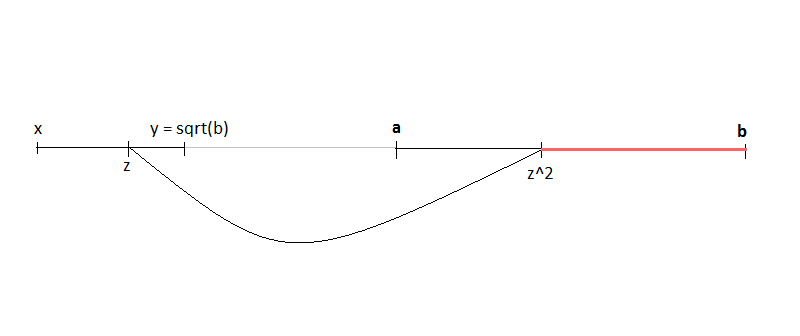
\includegraphics[width=\textwidth]{img/erat.png}
\caption{}
\end{figure}

Elég $\sqrt{b}$-ig felmennünk a szitatábla felső korlátjával. Ahhoz, hogy ezt belássuk, vegyük észre, hogy minden a szitatáblában lévő, prímmel csak annak négyzetétől kell kezdenünk szitálni. \par 
Jelöljük a szitatáblát [x,y]-nal. Ekkor legyen $x < z < y$. Ekkorra már kiszitáltunk minden x és z közé eső prímmel. Vagyis azok a számok, amelyek oszthatóak valamely $z$-nél kisebb prímmel, már ki vannak szitálva. Vagyis az első olyan szám, amit vizsgálnunk kell, az a $z^2$. \par
Ebből már jól látszódik, egrészt az, hogy a fenti jelölést használva $y=\sqrt{b}$, másrészt ahogy haladunk előre a szitálóprímekkel, a vizsgált intervallum egyre kisebb lesz. Ez az egyszerűsítés rengeteget javít a program teljesítményén. Tfh. hogy $[x,y]=[10^6,4\cdot10^6]$. Ekkor a naív $4\cdot10^6$ szitatábla méret helyett elég mindössze $\sqrt{4\cdot10^6}=2000$ méretű tábla.
\item Legyen \textit{p} a szitatábla első eleme, a legkisebb prím: 2.
\item Jelöljük meg \textit{p} összes többszörösét a vizsgált intervallumban, kedzve $p^2$-től, ha $a<p^2 $. \label{szita}
\item Legyen \textit{p} a szitatábla következő eleme, a következő szitáló prím. Ha nincs ilyen akkor vége az algoritmusnak. Ha van ilyen, akkor folytassuk a \ref{szita}. ponttal.
\end{enumerate}

\begin{figure}[h]
\centering
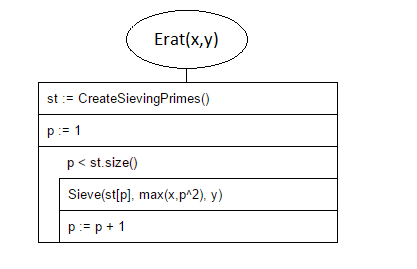
\includegraphics{img/erat_stuki.png}
\caption{Erathosztenészi-szita}
\end{figure}

\bigskip
Az iteráció végén a jelöletlenül maradt számok lesznek a keresett prím számok. Ha egy ilyen szám összetett lenne, akkor már biztosan meg lett volna jelölve, hiszen a számelmélet alaptétele szerint felírható kisebb prímszámok szorzataként, vagyis egy kisebb prímszámnak a többszöröse, amikkel pedig már szitáltunk.
 \subsubsection{Hátrányok} \label{badbad}
Az algoritmus kisebb intervallumokra nagyon jól használható. A dolgozat során elvégzett mérések szerint körülbelül $2^17$-es nagyságrendig tartotta a lépést a később szóba kerülő COLS algoritmussal. De igazából algoritmikus módszerekkel nehéz tovább gyorsítani ezt a módszert. A nem prím számok kiszitálását nem tudjuk megúszni. \par
Viszont közismert tény, hogy a memória műveletek nagyságrendekkel lassabbak, mint ahogy egy processzor képes végrehajtani műveleteket a már meglévő, a cache memóriában tárolt adatokon. És itt jön ki igazából a nagy hátránya az Erathosztenészi-szitának. Mi történik akkor, ha akkora intervallumot akarunk vizsgálni, amekkora nem fér be a memóriába? \par
TODO: insert ábra \par
Ahogy az ábrán is látszódik, ilyen esetben nem tudunk végigszitálni egy adott kis prímmel az egész intervallumon. Amint elérjük a cache "végét", nem fogja találni a keresett következő számot a program, ezt hívják \textbf{cache miss}nek. Ilyenkor be kell kérni a hiányzó adatot jó esetben a RAM memóriából, rosszabb esetben a háttértárról. Ráadásul, amint kiszitáltunk egy prímmel, kezdhetjük beolvasni előről az összes adatot, jó esély van rá, hogy a processzor már kidobda az intervallum elején kiszitált számokat. Vagyis ez azt jelenti, hogy legrosszabb esetben az intervallum összes számát újra és újra be kell olvasni, egészen pontosan $\sqrt{b}$-szer. Mondani sem kell, hogy ez mennyire lelassítja az program teljesítményét. Sejteni lehet, hogy a vizsgált intervallum növekedésével nem egyenesen arányos a program futásának ideje. Ezt később be is látjuk majd, lásd: \ref{benchmark}

\subsection{Szegmensenkénit szitálás}

A \ref{badbad} fejezetben látott hátrányt mindenképp ki kell küszöbölni, ha valós környezetben is alkalmazható alkalmazást implementálni. Ugyanis a naív Erathosztenészi-szita nagyobb számok illetve intervallumok esetében az idő nagy részében a memóriából fog olvasni. Ez a probléma csak akkor fog jól látszódni, ha már akkora intervallumot szitálunk, ami nem fér bele a cache memóriába. Ez azért fordul elő, mert egyesével vesszük ki a prímeket a szitatáblából, és utána egyesével dolgozunk velük. Viszont ha megfordítanánk az algoritmust, és az intervallumból vennénk ki egy darabot, és ezzel dolgoznánk a szitatáblán, akkor megoldódna minden memória problémánk. Ugyanis a szitatábla mindössze $\sqrt{b}$ méretű, ami valószínűleg könnyedén elfér a lokális memóriában. \par 
Az előbb említett darabot, amit kiveszünk az intervallumból nevezzük szegmensnek, vagy angolul \textit{chunk}-nak. Ötlet: daraboljuk fel az egész intervallumot ilyen szegmensekre, és ezeket egyesével szitáljuk ki teljesen, majd írjuk vissza a memóriába. Így elérhetjük, hogy minden vizsgált szám mindössze egyszer kerüljön beolvasásra, nagyságrendekkel redukálva így a memória olvasások és írások számát. \par
Így tehát az algoritmus: \par
\begin{enumerate}
\item Készítsük el a kisebb prímekből alló szitatáblát a naív algoritmushoz hasonló módon.
\item Daraboljuk fel a vizsgált intervallumot alkalmasan sok szegmensre. Ara, hogy pontosan mennyire finom felosztás a legjobb választás nem lehet általánosan jó választ adni. Függ a használt számítógép specifikációjától. Valamint természetesen egy számítógép közben sok más dologra is használja a cache memóriáját, így nem lehet előre egy legjobb felosztást mondani. Ráadásul ha túl finom felosztást választunk, akkor pedig lehet, hogy csak felesleges overheadet okozunk a programnak. \par
Viszont kisebb, de már elég nagy példákon kísérletezve be lehet lőni azt, hogy körülbelül mi lenne a legmegfelelőbb felosztás.
\item Olvassuk be az első szegmenst a memóriába.
\item Legyen \textit{p} a szitatábla első eleme. \label{chunkszita}
\item Jelöljük meg \textit{p} összes többszörösét a beolvasott szegmensben, kezdve $p^2$-től, ha $a<p^2$.
\item Legyen \textit{p} a szitatáblából a következő szitáló prím. Ha nincs ilyen, akkor kész vagyunk az aktuális szegmens kiszitálásával, vagyis már akár ebből a szegmensből ki is lehetne olvasni a benne lévő prím számokat. Ekkor olvassuk be a következő szegmenst, és folytassuk a \ref{chunkszita}-es ponttal. \par
Ha viszont nincs több szegmens, akkor készen vagyunk, vége az algoritmusnak. 
\end{enumerate}

\begin{figure}[h]
\centering
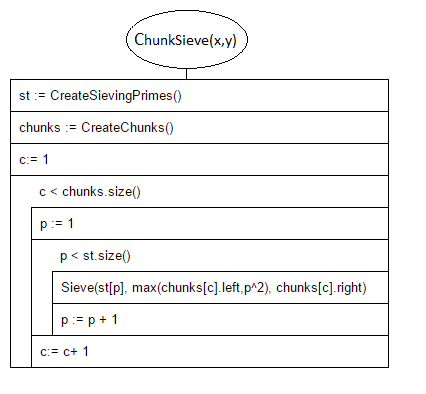
\includegraphics{img/chunk_stuki.png}
\caption{Szegmensenkéni szitálás}
\end{figure}

Amint később látni fogjuk, csak ezzel a módosítással volt, hogy több mint 3-szoros sebesség növekedést lehetett elérni. Lásd: \ref{benchmark}
\subsection{COLS} \label{cols}

\clearpage
\section{Felhasználói dokumentáció}

\subsection{A program használata} \label{usage}

A programot a \textbf{/source/soe.exe} binálris indításával tudjuk futtatni. Ha mást nem adtunk meg, akkor bemenetként a \textit{/source/utils/config1.txt/} fájlt fogja felhasználni. Ha véget ért a futás, akkor a program a \textbf{/result/} mappába fogja elhelyezni a kiszámolt prímeket a \textit{result.txt} fájlba, ha mást nem adtunk meg.\par \bigskip
Lehetőségünk van azonban befoláysolni a program futását konfigurációs fájlokkal. Ezeket a \textit{/source/utils/} mappába kell létrehozni, és a következő sémát kell követniük:
\begin{itemize}
\item lower bound: a
\item upper bound: b
\item max number of chunks: c
\item number of threads: t
\end{itemize}
Ahol \([a,b]\) a kiszitálni kívánt intervallum, \textit{c} a szegmensek maximális száma (ezt bizonyos esetekben csökkentheti a program, lásd: \ref{program}) és t a használt szálak száma. \par
\bigskip
Tehát amennyiben szeretnénk a saját konfigurációs fájlunkat használni, azt a programnak bementi paraméterként kell megadnunk. Hasonlóan azt is, ha a kimeneti féjlt szeretnénk megváltoztatni. \par \bigskip
soe.exe [config] [result] \par
Például: soe.exe myConfig.txt myResult.txt

\subsection{Rendszerkövetelmények}

A program 64-bites Microsoft Windows operációs rendszer használatával íródott és lett tesztelve. (Windows 7 és 10) Így az ilyen operációs rendszereken biztosan helyesen működik. \par
Ahhoz, hogy UNIX alapú operációs rendszeren, illetve 32-bites rendszereken használni tudjuk, ahhoz újra kell fordítani a programot. Lásd: \ref{build} Ezeken a rendszereken nem lett tesztelve a program, de nem használja ki a használt operációs rendszer által nyújtott lehetőségeket, ezért portolható. De természetesen ajánlott a tesztelő program használata is más rendszereken való használat előtt.

\subsection{CD tartalma, telepítés}

A \textit{docs} mappában található a programhoz tartozó dokumentáció .pdf formátumban. \par
A \textit{source} mappában található a futtatható fájl, ennek neve sieve.exe. Ezt a fájlt futtatva indíthatjuk el a programot. Ebben a mappában találhatóak továbba a program forrásfájljai is.  A program konfigurálásához lásd: \ref{usage}. A program módosításához, illetve újrafordításához lásd: \ref{build} \par
A program teszteléséhez használt fájlok a \textit{test} mappában találhatóak. Bővebben lásd: \ref{test} \par
A \textit{result} mappába helyezi el a program a kiszámított eredményeket. Természetesen a CD-re nem tud írni a program. \par
A \textit{benchmark} mappában találhatóak a programban elkészített algoritmusok segítségéhez használt fájlok. Itt található még korábbi mérési eredmények benchmark\_result\_dátum.xlsx néven. \bigskip

\noindent \underline{Telepítés:} \par
A program használható közvetlenül a CD-ről is, bár ekkor nem tudjuk a kapott ererdményeket megteinteni. Ehhez a CD tartalmát másoljuk fel a használni kívánt számítógépre, és ezek után a program a fentebb említett \textit{result} mappába fogja másolni az eredményeit.

\clearpage
\section{Fejlesztői dokumentáció}

\subsection{Felhasznált technológiák}
A program C++ programozási nyelv standard C++11-es verziójának használatával íródott. Semmilyen külső könyvtárat nem használ, így könnyen újrafordíthatja és portolhatja más rendszerre bárki. \par
A párhuzamos szálakon történő futtatáshoz a standard C++11 által kínált \textbf{thread} könyvtár van felhasználva. \par
A program fejlesztése során a verziókövetésre a GitHub online verziókövető rendszer volt használva. Egy program implementációja során kiemelten fontos egy hasonló szolgáltatás használata. Ennek segítségével könnyedén nyomon lehet követni a program fejlesztésének történetét, és egyszerűen lehet több számítógépről is folytatni a fejlesztést. A program megtalálható az alábbi helyen: https://github.com/peterhuszti/Thesis-MSc \par
A program tesztelése szintén standard C++ segítsgével lett megoldva. A dolgozat során ahol lehetett próbáltam a C++11-es szabvány által nyújtott lehetőségeket kihasználni. Erre jó példa a thread könyvtár használata, ami egy nagyon egyszerű API-t kínál szálak definiálására és általában konkurens programok készítésére. Továbba ki van hasnzálva a C++-ban újdonságnak számító lambda kifejezések ereje is. Ezeknek a lambdáknak, vagy más néven névtelen eljárásoknak a különlegessége, hogy nem tartozik hozzájuk azonosító. Ezeket felhasnzálva egyszerűen tudunk eljárásokat paraméterül adni magasabb rendű függvényeknek, például szálak viselkedésének a megadásakor. \par
A benchmark elkészítéséhez a Benchpress nevű frameworköt használtam. Ez egy nagyon egyszerűen és könnyen használható eszköz, amivel C++11 nyelven írt programok, vagy akár csak külön függvények és eljárások futási sebességét lehet mérni. REF \par

\subsection{Fordítás} \label{build}

Ahhoz, hogy le tudjuk újra fordítani a programot, ahhoz egy C++11 kompatibilis fordítóra van szükség. A program eredetileg a g++ 5.2.0-ás verziójával lett lefordítva, de semmi akadálya annak, hogy más megfelelő fordítóprogramot használjunk. \par
Ha viszont g++-t használunk, akkor a következő javasolt g++ [-o sieve] -O3 -std=c++11 main.cpp. Az -o kapcsoló nem szükséges, ezzel csupán az elkészített futtatható fájl nevét tudjuk megadni. Az -std=c++11 paraméterrel tudjuk megadni, hogy a fordító a C++11-es szabvány szerint próbálja meg lefordítani a programot. Az -O3 paraméter egy optimalizációs paraméter. Ezekről bővebben lásd: \ref{optpar}

\subsection{A program felépítése} \label{program}

A program belépési pontja a \textbf{/source/main.cpp}. Az összes többi forrásfájl a \textbf{/source/utils/} mappában található. \par \bigskip
Az \textbf{utils.h} fájl tartalmazza a konfigurációs fájlok beolvasását, valamint a program futását vezérlő \textit{start()} metódust. \par \bigskip
A \textbf{Printer.h} féjlban található \textit{Printer} osztály segítségével tudunk kiíratni minden adatot a program futásáról, valamint ez az osztály készíti el a megoldás fájlt is. Fontos volt külön kezelni ezt magától a konkrét számolástól, mert nem tartozik szorosan a feladat megoldásához, így logikailag is külön egységet alkotnak. A \textit{Printer} osztály a később említett \textit{Siever} osztály ún. barát osztálya, ami azt jelenti, hogy minden privát adattagját el tudja érni. \par \bigskip
Végül, de nem utolsó sorban itt található még a \textbf{Siever.h} fájl, benne a \textit{Siever} osztállyal, ami az összes számítás elvégzéséért felelős. \par

A továbbiakban részletesebben ismertetve lesznek ezen osztály adattagjai és metódusai.
\begin{itemize}
\item \textit{last\_number}: a fenti jelölések szerint $y=\sqrt{b}$, vagyis a szitatábla utolsó száma. \par Ehhez kapcsolódik a \textit{log\_upper\_bound} adattag is, amire igaz, hogy: 
\( 2^{log\_upper\_bound}-1=last\_number \)
\item \textit{size\_of\_st}: a szitatábla mérete gépi szavakban. Viszont a szitatábla a legritkább esetben lesz csak pont a gépi szó méretének egész számú többzöröse, ezért szükségünk van arra is, hogy pontosabban, bitekben mérve mekkora helyet foglal a tábla, erre szolgál az \textit{nbits} adattag.
\item Hasonlóan a két fentebb említetthez van létrehozva a \textit{chunk\_size} és a \textit{chunk\_bits} adattag, amik a szegmensek méretére vonatkoznak.
\item \textit{chunk\_base}: az első vizsgált szám pozíciója
\item \textit{chunk\_per\_thread}, \textit{plus\_one\_sieve}, az előbbi változó tárolja azt, hogy egy szálnak hány szegmenst kell kiszitálnia, míg utóbbi azt, hogy ha a szegmensek száma nem osztható a szálak számával, akkor hány threadnek kell még plusz egy szegmenst kisztiálnia.
\item \textit{number\_of\_circles}, \textit{number\_of\_bucket}: a körök illetve az edények száma.
\bigskip\bigskip\bigskip
\item A \textit{soe\_init()} metódus fogja elkészíteni a szitatáblát, vagyis 3-tól \textit{nbits}-ig meg fogja keresni az összetett számokat, és ezekhez a számokhoz tartozó biteket bebillenti 1-re. Szóval később azokkal a számokkal, vagy bitekkel kell szitálni majd, amik 0-k.
\begin{lstlisting}
	void soe_init()
	{
		prime_t p = 3; // first prime
		prime_t q = P2I(p); // index in st

		while (p * p < I2P(nbits)) // need to sieve only until sqrt(upper_bound)
		{
			while (GET(st,q)) q++; // search the next 0 in st, i.e. the next prime to sieve with

			p = I2P(q); // what is this next sieving prime
			prime_t i = P2I(p*p); // need to sieve only from p^2 because the smallers are already sieved

			while (i < nbits) // sieve until it is in st
			{
				SET(st,i); // mark as composite
				i += p; // step forward p
			}
			q++; // step forward 1, so the 2. while can find the next prime to sieve with
		}
	} 
\end{lstlisting}
\item Az \textit{init\_offsets}, \textit{init\_buckets} és a \textit{init\_circles} metódusok a probléma inicializálására szolgálnak. Lásd: \ref{cols}
\begin{lstlisting}
	void init_buckets(const std::vector<Params_for_threads> &params)
	{
		init_offsets(params);
	
		for (size_t j=0; j<number_of_threads; ++j) // for all threads
		{
			buckets[j][0] = circles[0];
		
			size_t p = 0;
			size_t b = 1;
			for (circle_t circle_id=1; circle_id<number_of_circles; ++circle_id)
			{
				word_t temp = chunk_bits;
				for (bucket_t bucket_id=0; bucket_id<circle_id+1; ++bucket_id)
				{
					for (; p < circles[circle_id] && st_pairs[j][p].offset < temp; ++p) { }
					buckets[j][b++] = p-1;
					if (bucket_id != 0)
					{
						for (size_t i=buckets[j][b-1]+1; i<=buckets[j][b]; ++i)
						{
							st_pairs[j][i].offset -= chunk_bits;
						}
					}
					temp += chunk_bits;
				}
			}		
		}
	}
\end{lstlisting}
\item Az \textit{update\_offsets} és az \textit{update\_buckets} metódusok minden edénnyel való szitálás után újrarendezik az edényeket, lásd \ref{cols}
\begin{lstlisting}
	void update_buckets(size_t thread_id)
	{
		for (circle_t circle_id=0; circle_id<number_of_circles; ++circle_id)
		{
			auto actual_bucket = get_actual_bucket(thread_id, circle_id);
			bool stay = false;
			bucket_t index = actual_bucket.first;
			bucket_t end = actual_bucket.second;
			while (!stay && index <= end)
			{
				stay = st_pairs[thread_id][index].offset < chunk_bits;
				index++;
			}
			bucket_t first_bucket_in_circle = circle_id*(circle_id+1)/2;
			buckets[thread_id][first_bucket_in_circle] = index-1;
			
			bucket_t last_bucket_in_circle = first_bucket_in_circle + circle_id;
			bucket_t temp = buckets[thread_id][last_bucket_in_circle];
			for (bucket_t bucket_id=last_bucket_in_circle; bucket_id>first_bucket_in_circle+1; --bucket_id)
			{
				buckets[thread_id][bucket_id] = buckets[thread_id][bucket_id-1];
			}
			buckets[thread_id][first_bucket_in_circle+1] = temp;
		}	
	}
\end{lstlisting}
\end{itemize}

\begin{figure}[h]
\centering
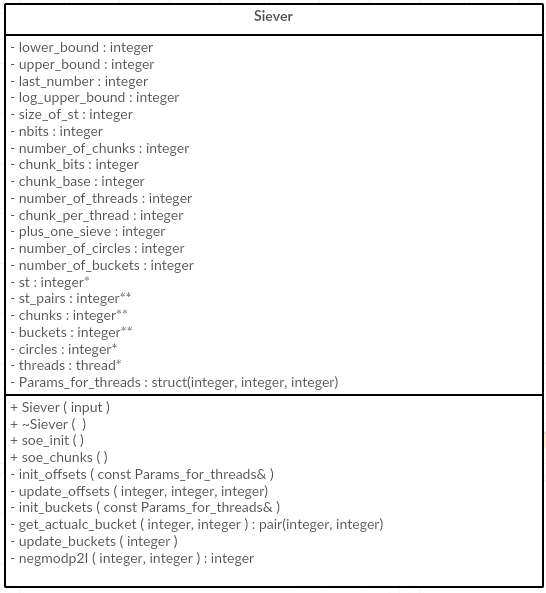
\includegraphics{img/siever.png}
\caption{Siever osztály}
\end{figure}

\clearpage
\subsection{Adatszerkezetek}

\subsubsection{Szitatábla, szegmensek}

A szitatáblával, valamint a vizsgált intervallummal nem lenne hatékony a számítás, ha egy az egyben eltárolnánk a számokat. Mint ahogy korábban is volt róla szó, nagyon fontos, hogy a memória olvasások számát redukáljuk. Ebből kifolyólag egy számot egy bittel fogunk reprezentálni, és egy adott számot a pozíciója alapján fogunk beazonosítani. Ennek eléréséhez vannak definiálva a következő preprocesszor makrók: INDEX, MASK, GET, SET, RESET, P2I, I2P, valamint a LOG\_WORD\_SIZE, ami az egy gépi szót határozza meg, vagyis \par
\( gepi\_szo = 2^{LOG\_WORD\_SIZE} \). Fontos észrevenni még, hogy a páros számokat nem muszáj tárolni. Könnyedén figyelembe lehet venni a bitek maszkolásánál ezt, és így még megfeleztük a tárolt számok összméretét- \par
Így például egy 64 bites rendszeren az eltárolt számok 1/128-ednyi memóriát fognak foglalni. \par
Éppen ezért ezek táblák pointerekként vannak definiálva, amivel meg van határozva a legelső elemük. Innentől kezdve már csak azt kell kiszámolni, hogy az aktuális szám hanyadik a táblában, vagyis hány bit távolságra van a kezdőponthoz képest. \par
\bigskip
A szegmensek a szitatáblához hasonlóan vannak ábrázolva és eltárolva, minden számot egy bit reprezentál. Tárolva van a legelső szegmens első száma, valamint az, hogy hány bitből áll egy adott szegmens, így könnyedén ki lehet számolni a szegmensek határait.

\subsubsection{Körök és edények}

A körök és az edények alkotják a COLS algoritmus lényegét. Ezek egyszerű mutatóként vannak reprezentálva, amik megadják, hogy a szitatáblában az adott körök és edények meddig tartanak, vagyis mi az utolsó elemük. \par
Amíg körök fixek és adottak, addig a körök dinamikusan változnak a program futása során, minden szálon külön-külön. Vagyis minden sázl birtokol és karbantart egy-egy edény tömböt. \par
A könnyeb implementáláshoz létre lett hozva egy \textit{st\_pairs} tömb minden szálra. Ezek atömbök tartalmazzák prímek indexeit, valamint az aktuális, az adott szegmensbe való offsetüket, vagyis, hogy hova kell szitálniuk először az adott szegmensbe. 

\subsection{Párhuzamos megvalósítás, skálázhatóság} \label{scale}



\subsection{Tesztelés} \label{test}

A tesztelést a \textbf{/test/} mappában található fájlok oldják meg. Egy fajta teszt létezik a programhoz, mégpedig egy rendszer teszt. Ez azt vizsgálja, hogy az adott paraméterekkel indított szitáló algoritmus megtalálja-e a megfelelő prímszámokat, és csak azokat találja-e meg. Ehhez szükség van egy referencia megoldásra, amit a \textit{/test/primes.txt} szövegfájlban találhatunk. \par
 Tartozik a tesztelő programhoz egy \textit{Testcase\_generator} osztály is, ami elkészíti a beállításoknak megfelelő teszteket. A tesztelő programban be lehet állítani, hogy melyik intervallumot szitálja, valamint a használt szegmens szám és szál számokra egy intervallum, amiben a generátor legyártja a köztes teszteseteket, amit majd a tesztelő fog futtatni.

\clearpage
\section{Az algoritmusok összehasonlítása}

\subsection{Használt hardverek}

A dolgozat során kettő konfiguráción volt lehetőség tesztelni a program és az algoritmusok sebességét és teljesítményét: \bigskip \bigskip \bigskip

'A' konfiguráció ~~~~~~~~
\begin{tabular}{ | c | }
  \hline
  Intel Core i5-5300U @ 2.3GHz \\ \hline
  2 core, 4 thread \\ \hline
  3 MB cache \\ \hline
  Max. memória sávszélesség: 25.6 GB/s \\ \hline
  8 GB RAM\\ \hline
  64-bit Windows 7 \\
  \hline
\end{tabular}

\bigskip \bigskip

'B' konfiguráció ~~~~~~~~
\begin{tabular}{ | c | }
  \hline
  Intel Core i7-4790 @ 3.6GHz \\ \hline
  4 core, 8 thread \\ \hline
  8 MB cache \\ \hline
  Max. memória sávszélesség: 25.6 GB/s \\ \hline
  16 GB RAM\\ \hline
  64-bit Windows 10 \\
  \hline
\end{tabular}

\bigskip \bigskip

Érdemes megjegyezni, hogy az 'A' konfiguráció egy laptop, míg a 'B' egy asztali számítógép. Később jól fog látszódni a két számítógép közötti teljesítmény különbség. \par
Korábban volt szó a skálázhatóságról, lásd \ref{scale}. Érdekes lenne kipróbálni egy nagyobb, több processzort tartalmazó konfiguráción is a programot, de erre sajnos a dolgozat készítése során nem volt lehetőség.

\subsection{Fordítási paraméterek} \label{optpar}

\subsection{Az eredmények} \label{benchmark}

\subsection{Konklúzió}

\clearpage
\section{Összegzés}

\end{document}







































